\documentclass{article}
\usepackage{arxiv}

\usepackage[utf8]{inputenc}
\usepackage[english, russian]{babel}
\usepackage[T1]{fontenc}
\usepackage{url}
\usepackage{booktabs}
\usepackage{amsfonts}
\usepackage{nicefrac}
\usepackage{microtype}
\usepackage{lipsum}
\usepackage{graphicx}
\usepackage{natbib}
\usepackage{doi}

\usepackage{url}
\usepackage{wrapfig,booktabs}
\usepackage{titlesec}
\usepackage[inkscapeformat=png]{svg}
\usepackage{adjustbox}
\usepackage{caption}
\usepackage{subcaption}
\usepackage{graphicx}
\usepackage{multirow}

\usepackage{algorithm}
\usepackage{algpseudocode}
\usepackage{amsfonts}
\usepackage{amssymb, amsmath, mathrsfs, amsthm}
\usepackage{bbm}
\usepackage{bm}
\usepackage{color}
\usepackage{csvsimple}
\usepackage{fancyvrb}
\usepackage{indentfirst}
\usepackage{listings}
\usepackage{mathtools}
\usepackage{pgfplots}


\title{Разработка эффективной реализации методов, основанных на поиске оптимального баланса между дивергенцией и точностью аппроксимации}

\author{ Аристархов Данила Дмитриевич \\
	ВМК МГУ \\
	\texttt{aristarkhov.danila@yandex.ru} \\
	%% examples of more authors
	\And
	Сенько Олег Валентинович \\
	ВМК МГУ \\
	\texttt{senkoov@mail.ru} \\
}
\date{}

\renewcommand{\shorttitle}{\textit{arXiv} Template}

%%% Add PDF metadata to help others organize their library
%%% Once the PDF is generated, you can check the metadata with
%%% $ pdfinfo template.pdf
\hypersetup{
pdftitle={},
pdfsubject={q-bio.NC, q-bio.QM},
pdfauthor={Аристархов Д.Д., Сенько О.В.},
pdfkeywords={регрессия, коллективные методы, бэггинг, градиентный бустинг},
}

\begin{document}
\maketitle

\begin{abstract}
	Рассмотрен новый метод построения ансамбля деревьев при решении задачи регрессии. При этом оптимизация производится исходя из одновременного достижения расходимости алгоритмов в пространстве прогнозов и хорошей аппроксимации данных отдельными алгоритмами ансамбля. 
\end{abstract}


\keywords{регрессия \and коллективные методы \and бэггинг \and градиентный бустинг}

\section{Введение}

Методы решения задачи регрессии, основанные на вычислении более точного предсказания с помощью набора менее точных и более простых базовых алгоритмов, получили самое широкое распространение в современном машинном обучении. К числу таких методов может быть отнесен регрессионный случайный лес, а также методы, основанные на использовании адаптивного или градиентного бустинга. Важную роль при построении таких алгоритмов играет способ получения ансамбля так называемых слабых алгоритмов. Теоретический анализ показывает, что увеличение обобщающей способности может быть достигнуто за счет выбора ансамбля алгоритмов, обладающих не только высокой точностью, но и максимально расходящимися прогнозами \citep{convex}. В случайном лесе расходимость прогнозов достигается за счет обучения алгоритмов ансамбля на различных выборках, генерируемых из исходной выборки с использованием процедуры бутстрэпа \citep{bagging}. В методе градиентного бустинга \citep{boosting} ансамбль генерируется последовательно. При этом на каждой итерации в ансамбль добавляются деревья, аппроксимирующие первые производные функции потерь в точке, соответствующей текущему прогнозу алгоритма на данном шаге.

Построение ансамбля, имеющего как высокую точность предсказаний, так и сильное расхождение прогнозов отдельных алгоритмов, продемонстрировало улучшение качества модели \citep{twolevel}. Целью данной работы является продолжение исследования данного подхода.

\section{Постановка задачи}
Дана выборка $S={(X_1, y_1), \dots, (X_m, y_m)}$, где $X_i$ --- вектор признакового описания объекта, $y_i$ --- метка объекта. Рассматривается задача регресии: $X_i~\in~\mathbb{R}^n, \  y_i \in \mathbb{R}$. Требуется построить ансамбль базовых алгоритмов $A_1(X), \dots, A_k(X)$, предсказывающих значения метки по вектору признаков.

\section{Дисперсия ансамбля}
Рассмотрим известное разложение среднеквадратичного риска модели $\mu(x)$ (bias-variance decomposition):
\begin{equation*}
  L(\mu) = N(\mu) + B(\mu) + V(\mu),
\end{equation*}
где
\allowdisplaybreaks
\begin{align*}
  N(\mu) &= \mathbb{E}_{x, y} \Bigl[\bigl(y - \mathbb{E}[y | x] \bigr)^2\Bigr] \text{ --- шум,} \\
  B(\mu) &= \mathbb{E}_{x} \Bigl[
            \bigl(
                \mathbb{E}_{X} \bigl[ \mu(X) \bigr]
                -
                \mathbb{E}[y | x]
            \bigr)^2
        \Bigr] \text{ --- смещение,} \\
  V(\mu) &= \mathbb{E}_{X} \Bigl[
                \bigl(
                    \mu(X)
                    -
                    \mathbb{E}_{X} \bigl[ \mu(X) \bigr]
                \bigr)^2
            \Bigr] \text{ --- разброс.}
\end{align*}

Проанализируем это разложение в случае ансамбля базовых алгоритмов $\mu(X) = \frac{1}{k} \sum_{i=1}^{k} A_i(X)$. Шум является свойством выборки и не зависит от алгоритма. Выражения для смещения принимает вид:

\begin{align*}
    B(\mu) &= \mathbb{E}_{x, y} \Bigl[
        \Bigl(
            \mathbb{E}_{X} \Bigl[
                \frac{1}{k}
                \sum_{i = 1}^{k}
                    A_i(X)(x)
            \Bigr]
            -
            \mathbb{E}[y | x]
        \Bigr)^2
    \Bigr]
    =\\
    &=
    \mathbb{E}_{x, y} \Bigl[
        \Bigl(
                \frac{1}{k}
                \sum_{i = 1}^{k}
                    \mathbb{E}_X[ A_i(X)(x) ]
            -
            \mathbb{E}[y | x]
        \Bigr)^2
    \Bigr]
    =\\
    &=
    \mathbb{E}_{x, y} \Bigl[
        \bigl(
            \mathbb{E}_{X} \bigl[
                A_i(X)(x)
            \bigr]
            -
            \mathbb{E}[y | x]
        \bigr)^2
    \Bigr].
\end{align*}
Таким образом, ансамблирование не изменяет смещенности относительно базового алгоритма.

Запишем выражения для разброса ансамбля:
\begin{align*}
  V(\mu) &= \mathbb{E}_{x, y} \Bigl[
    \mathbb{E}_{X} \Bigl[
      \Bigl(
        \frac{1}{k}
        \sum_{i = 1}^{k}
        A_i(X)(x)
        -
        \mathbb{E}_{X} \Bigl[
          \frac{1}{k}
          \sum_{i = 1}^{k}
          A_i(X)(x)
          \Bigr]
          \Bigr)^2
          \Bigr]
          \Bigr] \\
    &= \mathbb{E}_{x, y} \Bigl[
    \mathbb{E}_{X} \Bigl[
    \frac{1}{k^2}
    \Bigl(
        \sum_{i = 1}^{k} \Bigl[
                A_i(X)(x)
                -
                \mathbb{E}_{X} \bigl[
                    A_i(X)(x)
                \bigr]
        \Bigr]
    \Bigr)^2\Bigr]
          \Bigr]
    =\\
    &= \mathbb{E}_{x, y} \Bigl[
    \mathbb{E}_{X} \Bigl[
    \frac{1}{k^2}
    \sum_{i = 1}^{k} \Bigl(
        A_i(X)(x)
        -
        \mathbb{E}_{X} \bigl[
            A_i(X)(x)
        \bigr]
    \Bigr)^2 +\\
    &\text{\hspace{0.5cm}}+
    \frac{1}{k^2}
    \sum_{i \neq j} \Bigl(
        A_i(X)(x)
        -
        \mathbb{E}_{X} \bigl[
            A_i(X)(x)
        \bigr]
    \Bigr)
    \Bigl(
        A_j(X)(x)
        -
        \mathbb{E}_{X} \bigl[
            A_j(X)(x)
        \bigr]
    \Bigr)\Bigr]
          \Bigr] \\
    &=
    \frac{1}{k^2}
    \mathbb{E}_{x, y} \Bigl[
        \mathbb{E}_{X} \Bigl[
            \sum_{i = 1}^{k} \Bigl(
                A_i(X)(x)
                -
                \mathbb{E}_{X} \bigl[
                    A_i(X)(x)
                \bigr]
            \Bigr)^2
        \Bigr]
    \Bigr]
    +\\
    &\text{\hspace{0.5cm}}+
    \frac{1}{k^2}
    \mathbb{E}_{x, y} \Bigl[
        \mathbb{E}_{X} \Bigl[
            \sum_{i \neq j} \Bigl(
                A_i(X)(x)
                -
                \mathbb{E}_{X} \bigl[
                    A_i(X)(x)
                \bigr]
            \Bigr) 
            \Bigl(
                A_j(X)(x)
                -
                \mathbb{E}_{X} \bigl[
                    A_j(X)(x)
                \bigr]
            \Bigr)
        \Bigr]
    \Bigr]
    \\
    &=
    \frac{1}{k}
    \mathbb{E}_{x, y} \Bigl[
        \mathbb{E}_{X} \Bigl[
            \Bigl(
                A_i(X)(x)
                -
                \mathbb{E}_{X} \bigl[
                    A_i(X)(x)
                \bigr]
            \Bigr)^2
        \Bigr]
    \Bigr]
    +\\
    &\text{\hspace{0.5cm}}+
    \frac{k(k-1)}{k^2}
    \mathbb{E}_{x, y} \Bigl[
        \mathbb{E}_{X} \Bigl[
            \Bigl(
                A_i(X)(x)
                -
                \mathbb{E}_{X} \bigl[
                    A_i(X)(x)
                \bigr]
            \Bigr)
            \Bigl(   
                A_j(X)(x)
                -
                \mathbb{E}_{X} \bigl[
                    A_j(X)(x)
                \bigr]
            \Bigr)
        \Bigr]
    \Bigr]
\end{align*}
В данном разложении первое слагаемое~--- это дисперсия одного базового алгоритма,
деленная на длину композиции~$k$.
Второе~--- ковариация между двумя базовыми алгоритмами.
При малой коррелляции алгоритмов происходит существенное снижение разброса ансамбля по сравнению с базовым алгоритмом.

\section{Случайный лес} \label{sec:random_forest}
В качестве базового алгоритма в случайных лесах используются решающие деревья. Они имеют достаточную сложность, и, как следствие, низкую смещенность (при неограниченной глубине дерево может идеально подстроиться под выборку), но переобучаются и имеют высокий разброс, который можно уменьшить с помощью ансамблирования. В случайных лесах коррелляция между деревьями понижается двумя способами:
\begin{itemize}
  \item Бэггинг. Каждый алгоритм обучается на случайной подвыборке, сгенерированной из выборки с помощью бутстрэпа, т.е. выбираются $m$ объектов с возвращениями. Таким образом, в одной выборке некоторые объекты встретятся несколько раз, а некоторые — ни разу.
  \item Рандомизация признаков. При построении очередного дерева в каждой вершине выбор наилучшего признака для разбиения происходит не из всех возможных признаков, а из случайно выбранной подвыборки. 
\end{itemize}
Так удается добавить случайность в построение деревьев и уменьшить коррелированность их прогнозов.


% \section{Introduction}
% \lipsum[2]
% \lipsum[3]

% \section{Headings: first level}
% \label{sec:headings}

% \lipsum[4] See Section \ref{sec:headings}.

% \subsection{Headings: second level}
% \lipsum[5]
% \begin{equation}
% 	\xi _{ij}(t)=P(x_{t}=i,x_{t+1}=j|y,v,w;\theta)= {\frac {\alpha _{i}(t)a^{w_t}_{ij}\beta _{j}(t+1)b^{v_{t+1}}_{j}(y_{t+1})}{\sum _{i=1}^{N} \sum _{j=1}^{N} \alpha _{i}(t)a^{w_t}_{ij}\beta _{j}(t+1)b^{v_{t+1}}_{j}(y_{t+1})}}
% \end{equation}

% \subsubsection{Headings: third level}
% \lipsum[6]

% \paragraph{Paragraph}
% \lipsum[7]



% \section{Examples of citations, figures, tables, references}
% \label{sec:others}

% \subsection{Citations}
% Citations use \verb+natbib+. The documentation may be found at
% \begin{center}
% 	\url{http://mirrors.ctan.org/macros/latex/contrib/natbib/natnotes.pdf}
% \end{center}

% Here is an example usage of the two main commands (\verb+citet+ and \verb+citep+): Some people thought a thing \citep{kour2014real, hadash2018estimate} but other people thought something else \citep{kour2014fast}. Many people have speculated that if we knew exactly why \citet{kour2014fast} thought this\dots

% \subsection{Figures}
% \lipsum[10]
% See Figure \ref{fig:fig1}. Here is how you add footnotes. \footnote{Sample of the first footnote.}
% \lipsum[11]

% \begin{figure}
% 	\centering
% 	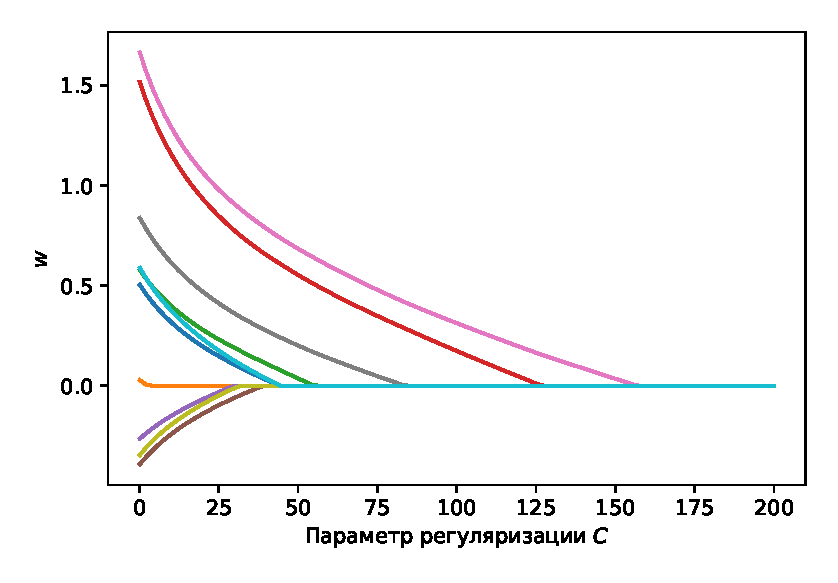
\includegraphics[width=0.5\textwidth]{../figures/log_reg_cs_exp.eps}
% 	\caption{Sample figure caption.}
% 	\label{fig:fig1}
% \end{figure}

% \subsection{Tables}
% See awesome Table~\ref{tab:table}.

% The documentation for \verb+booktabs+ (`Publication quality tables in LaTeX') is available from:
% \begin{center}
% 	\url{https://www.ctan.org/pkg/booktabs}
% \end{center}


% \begin{table}
% 	\caption{Sample table title}
% 	\centering
% 	\begin{tabular}{lll}
% 		\toprule
% 		\multicolumn{2}{c}{Part}                   \\
% 		\cmidrule(r){1-2}
% 		Name     & Description     & Size ($\mu$m) \\
% 		\midrule
% 		Dendrite & Input terminal  & $\sim$100     \\
% 		Axon     & Output terminal & $\sim$10      \\
% 		Soma     & Cell body       & up to $10^6$  \\
% 		\bottomrule
% 	\end{tabular}
% 	\label{tab:table}
% \end{table}

% \subsection{Lists}
% \begin{itemize}
% 	\item Lorem ipsum dolor sit amet
% 	\item consectetur adipiscing elit.
% 	\item Aliquam dignissim blandit est, in dictum tortor gravida eget. In ac rutrum magna.
% \end{itemize}


\bibliographystyle{unsrtnat}
\bibliography{references}

\end{document}